\iffalse
This file is protected by Copyright. Please refer to the COPYRIGHT file
distributed with this source distribution.

This file is part of OpenCPI <http://www.opencpi.org>

OpenCPI is free software: you can redistribute it and/or modify it under the
terms of the GNU Lesser General Public License as published by the Free Software
Foundation, either version 3 of the License, or (at your option) any later
version.

OpenCPI is distributed in the hope that it will be useful, but WITHOUT ANY
WARRANTY; without even the implied warranty of MERCHANTABILITY or FITNESS FOR A
PARTICULAR PURPOSE. See the GNU Lesser General Public License for more details.

You should have received a copy of the GNU Lesser General Public License along
with this program. If not, see <http://www.gnu.org/licenses/>.
\fi
%----------------------------------------------------------------------------------------
% Update the docTitle and docVersion per document
%----------------------------------------------------------------------------------------
\def\docTitle{IDE Guide}
\def\docVersion{1.2}
%----------------------------------------------------------------------------------------
\documentclass{article}
\iffalse
This file is protected by Copyright. Please refer to the COPYRIGHT file
distributed with this source distribution.

This file is part of OpenCPI <http://www.opencpi.org>

OpenCPI is free software: you can redistribute it and/or modify it under the
terms of the GNU Lesser General Public License as published by the Free Software
Foundation, either version 3 of the License, or (at your option) any later
version.

OpenCPI is distributed in the hope that it will be useful, but WITHOUT ANY
WARRANTY; without even the implied warranty of MERCHANTABILITY or FITNESS FOR A
PARTICULAR PURPOSE. See the GNU Lesser General Public License for more details.

You should have received a copy of the GNU Lesser General Public License along
with this program. If not, see <http://www.gnu.org/licenses/>.
\fi
\author{} % Force author to be blank
%----------------------------------------------------------------------------------------
% Paper size, orientation and margins
%----------------------------------------------------------------------------------------
\usepackage{geometry}
\geometry{
        letterpaper, % paper type
        portrait,    % text direction
        left=.75in,  % left margin
        top=.75in,   % top margin
        right=.75in, % right margin
        bottom=.75in % bottom margin
 }
%----------------------------------------------------------------------------------------
% Header/Footer
%----------------------------------------------------------------------------------------
\usepackage{fancyhdr} \pagestyle{fancy} % required for fancy headers
\renewcommand{\headrulewidth}{0.5pt}
\renewcommand{\footrulewidth}{0.5pt}
\rhead{\small{ANGRYVIPER Team}}
% \rfoot{\thepage}
%----------------------------------------------------------------------------------------
% Appendix packages
%----------------------------------------------------------------------------------------
\usepackage[toc,page]{appendix}
%----------------------------------------------------------------------------------------
% Defined Commands & Renamed Commands
%----------------------------------------------------------------------------------------
\renewcommand{\contentsname}{Table of Contents}
\renewcommand{\listfigurename}{List of Figures}
\renewcommand{\listtablename}{List of Tables}
%----------------------------------------------------------------------------------------
% Various packages
%----------------------------------------------------------------------------------------
\usepackage[usenames,dvipsnames]{xcolor} % for color names see https://en.wikibooks.org/wiki/LaTeX/Colors
\usepackage{hyperref}  % for linking urls and lists
\usepackage{graphicx}  % for including pictures by file
\usepackage{listings}  % for coding language styles
\usepackage{rotating}  % for sideways table
\usepackage{pifont}    % for sideways table
\usepackage{pdflscape} % for landscape view
\usepackage{subfig}
\usepackage{xstring}
\uchyph=0 % Never hyphenate acronyms like RCC (I think this overrides ANGRYVIPER above)
\renewcommand\_{\textunderscore\allowbreak} % Allow words to break/newline on underscores
%----------------------------------------------------------------------------------------
% Table packages
%----------------------------------------------------------------------------------------
\usepackage{longtable} % for long possibly multi-page tables
\usepackage{tabularx} % c=center,l=left,r=right,X=fill
% These define tabularx columns "C" and "R" to match "X" but center/right aligned
\newcolumntype{C}{>{\centering\arraybackslash}X}
\newcolumntype{R}{>{\raggedleft\arraybackslash}X}
\usepackage{float}
\floatstyle{plaintop}
\usepackage[tableposition=top]{caption}
\newcolumntype{P}[1]{>{\centering\arraybackslash}p{#1}}
\newcolumntype{M}[1]{>{\centering\arraybackslash}m{#1}}
%----------------------------------------------------------------------------------------
% Block Diagram / FSM Drawings
%----------------------------------------------------------------------------------------
\usepackage{tikz}
\usetikzlibrary{shapes,arrows,fit,positioning}
\usetikzlibrary{automata} % used for the fsm
%----------------------------------------------------------------------------------------
% Colors Used
%----------------------------------------------------------------------------------------
\usepackage{colortbl}
\definecolor{blue}{rgb}{.7,.8,.9}
\definecolor{ceruleanblue}{rgb}{0.16, 0.32, 0.75}
\definecolor{drkgreen}{rgb}{0,0.6,0}
\definecolor{deepmagenta}{rgb}{0.8, 0.0, 0.8}
\definecolor{cyan}{rgb}{0.0,0.6,0.6}
\definecolor{maroon}{rgb}{0.5,0,0}
%----------------------------------------------------------------------------------------
% VHDL Coding Language Style
% modified from: http://latex-community.org/forum/viewtopic.php?f=44&t=22076
%----------------------------------------------------------------------------------------
\lstdefinelanguage{VHDL}
{
        basicstyle=\ttfamily\footnotesize,
        columns=fullflexible,keepspaces,      % https://tex.stackexchange.com/a/46695/87531
        keywordstyle=\color{ceruleanblue},
        commentstyle=\color{drkgreen},
        morekeywords={
    library,use,all,entity,is,port,in,out,end,architecture,of,
    begin,and, signal, when, if, else, process, end,
        },
        morecomment=[l]--
}
%----------------------------------------------------------------------------------------
% XML Coding Language Style
% modified from: http://tex.stackexchange.com/questions/10255/xml-syntax-highlighting
%----------------------------------------------------------------------------------------
\lstdefinelanguage{XML}
{
        basicstyle=\ttfamily\footnotesize,
        columns=fullflexible,keepspaces,
        morestring=[s]{"}{"},
        morecomment=[s]{!--}{--},
        commentstyle=\color{drkgreen},
        moredelim=[s][\color{black}]{>}{<},
        moredelim=[s][\color{cyan}]{\ }{=},
        stringstyle=\color{maroon},
        identifierstyle=\color{ceruleanblue}
}
%----------------------------------------------------------------------------------------
% DIFF Coding Language Style
% modified from http://tex.stackexchange.com/questions/50176/highlighting-a-diff-file
%----------------------------------------------------------------------------------------
\lstdefinelanguage{diff}
{
        basicstyle=\ttfamily\footnotesize,
        columns=fullflexible,keepspaces,
        breaklines=true,                                % wrap text
        morecomment=[f][\color{ceruleanblue}]{@@},      % group identifier
        morecomment=[f][\color{red}]-,                  % deleted lines
        morecomment=[f][\color{drkgreen}]+,             % added lines
        morecomment=[f][\color{deepmagenta}]{---},      % Diff header lines (must appear after +,-)
        morecomment=[f][\color{deepmagenta}]{+++},
}
%----------------------------------------------------------------------------------------
% Python Coding Language Style
% modified from
%----------------------------------------------------------------------------------------
\lstdefinelanguage{python}
{
        basicstyle=\ttfamily\footnotesize,
        columns=fullflexible,keepspaces,
        keywordstyle=\color{ceruleanblue},
        commentstyle=\color{drkgreen},
        stringstyle=\color{orange},
        morekeywords={
    print, if, sys, len, from, import, as, open,close, def, main, for, else, write, read, range,
        },
        comment=[l]{\#}
}
%----------------------------------------------------------------------------------------
% Fontsize Notes in order from smallest to largest
%----------------------------------------------------------------------------------------
%    \tiny
%    \scriptsize
%    \footnotesize
%    \small
%    \normalsize
%    \large
%    \Large
%    \LARGE
%    \huge
%    \Huge

\date{Version \docVersion} % Force date to be blank and override date with version
\title{\docTitle}
\lhead{\small{\docTitle}}
%----------------------------------------------------------------------------------------
\begin{document}
\maketitle
\thispagestyle{fancy}
\newpage

	\begin{center}
	\textit{\textbf{Revision History}}
		\begin{table}[H]
		\label{table:revisions} % Add "[H]" to force placement of table
			\begin{tabularx}{\textwidth}{|c|X|l|}
			\hline
			\rowcolor{blue}
			\textbf{Revision} & \textbf{Description of Change} & \textbf{Date} \\
		    \hline
			v1.0 & Initial creation & 2/2016 \\
			\hline
			v1.1 & Updated for Release 1.1 & 3/2017 \\
			\hline
			v1.2 & Updated for Release 1.2 & 8/2017 \\
			\hline
			\end{tabularx}
		\end{table}
	\end{center}

\newpage

\tableofcontents

\newpage

\listoffigures

\newpage

\listoftables

\newpage

\section{References}

This document assumes a basic understanding of the Linux command line environment. It does not require a working knowledge of OpenCPI.
\def\refcapbottom{}
\iffalse
This file is protected by Copyright. Please refer to the COPYRIGHT file
distributed with this source distribution.

This file is part of OpenCPI <http://www.opencpi.org>

OpenCPI is free software: you can redistribute it and/or modify it under the
terms of the GNU Lesser General Public License as published by the Free Software
Foundation, either version 3 of the License, or (at your option) any later
version.

OpenCPI is distributed in the hope that it will be useful, but WITHOUT ANY
WARRANTY; without even the implied warranty of MERCHANTABILITY or FITNESS FOR A
PARTICULAR PURPOSE. See the GNU Lesser General Public License for more details.

You should have received a copy of the GNU Lesser General Public License along
with this program. If not, see <http://www.gnu.org/licenses/>.
\fi

% This snippet creates the "References" table labeled "table:references"
% It creates three columns: Name, Publisher, Link and then inserts default documents
%
% To skip these defaults, define macros named
% refskipgs to skip "Getting Started"
% refskipig to skip "Installation Guide"
% refskipac to skip "Acronyms and Definitions"
% refskipocpiov to skip "OpenCPI Overview"
%
% See RPM_Installation_Guide.tex for examples
%
% After the defaults, it optionally inserts the "myreferences" macro that
% you defined elsewhere (you put hlines above all lines)
%
% If you want the \caption on the bottom, define "refcapbottom"
\begin{center}
\renewcommand*\footnoterule{} % Remove separator line from footnote
\renewcommand{\thempfootnote}{\arabic{mpfootnote}} % Use Arabic numbers (or can't reuse)
\begin{minipage}{0.9\textwidth}
  \begin{table}[H]
\ifx\refcapbottom\undefined
  \caption {References}
  \label{table:references}
\fi
  \begin{tabularx}{\textwidth}{|C|C|}
    \hline
    \rowcolor{blue}
    \textbf{Title} & \textbf{Link} \\
\ifx\refskipocpiov\undefined
    \hline
    OpenCPI Overview & \githubio{Overview.pdf} \\
\fi
\ifx\refskipac\undefined
    \hline
    Acronyms and Definitions & \githubio{Acronyms\_and\_Definitions.pdf} \\
\fi
\ifx\refskipgs\undefined
    \hline
    Getting Started & \githubio{Getting\_Started.pdf} \\
\fi
\ifx\refskipig\undefined
    \hline
    Installation Guide & \githubio{RPM\_Installation\_Guide.pdf} \\
\fi
\ifx\myreferences\undefined
\else
    \myreferences
\fi
    \hline
  \end{tabularx}
\ifx\refcapbottom\undefined
\else
  \caption {References}
  \label{table:references}
\fi
  \end{table}
\end{minipage}
\end{center}

\newpage

\section{Document Overview}
\label{sec:doc_overview}
\begin{flushleft}
This document describes how to use the ANGRYVIPER IDE to modify existing OpenCPI assets as well as generate new assets in an Eclipse environment. The ANGRYVIPER Team's OpenCPI release includes an Eclipse package ready to read and generate OpenCPI asset files. The installation of the IDE is covered in the RPM Installation Guide. Once installed, the user can launch the IDE with the command \path{ocpigui}.
\end{flushleft}

\section{Create new OpenCPI Assets}
\label{sec:create_assets}
\begin{flushleft}

OpenCPI assets are created using an Eclipse wizard shown below. \newline
\begin{figure}[h!]
  \centering
  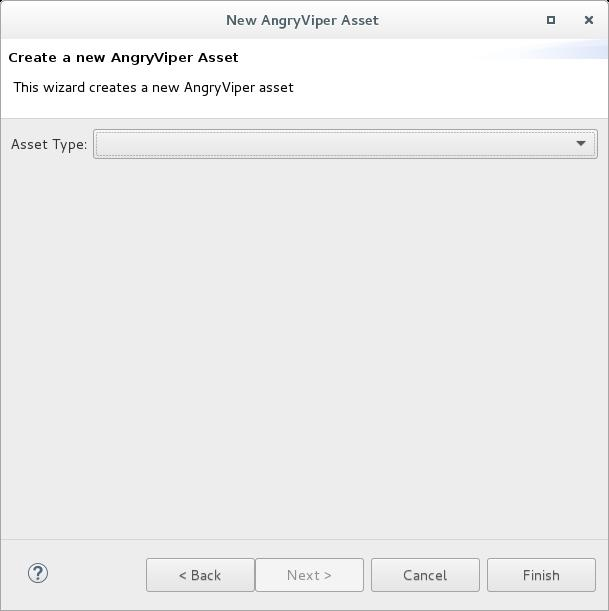
\includegraphics[scale=0.5]{figures/assetwizard.jpg}
  \caption{OpenCPI New Asset Wizard}
  \label{fig:figure1}
\end{figure}

The wizard allows you to choose which type of asset you wish to create and will dynamically update the available user input fields based upon that selection.  To access the wizard, select \textit{File --\textgreater New --\textgreater OpenCPI Asset}.

\end{flushleft}

\newpage

\subsection{Create New Project}
\label{sec:create_project}
\begin{flushleft}

To create an empty project for new assets select Project from the Asset Type drop-down list. Creating a new project requires the user to input a project name. There are also optional fields for a prefix, package name, and other projects the newly generated project will be dependent upon. This command generates a new Eclipse project in your current workspace where you can begin creating new assets.\newline
\begin{figure}[h!]
  \centering
  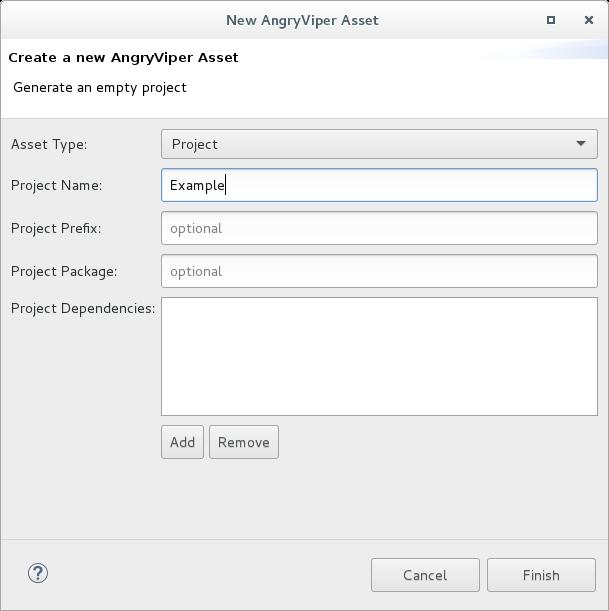
\includegraphics[scale=0.5]{figures/createproject.jpg}
  \caption{New OpenCPI Project Creation}
  \label{fig:figure2}
\end{figure}

\begin{figure}[h!]
  \centering
  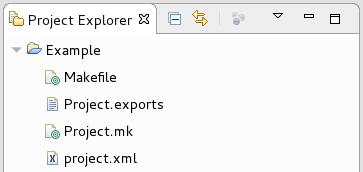
\includegraphics[scale=0.5]{figures/projectresult.jpg}
  \caption{Project Creation Result}
  \label{fig:figure3}
\end{figure}

\end{flushleft}

\newpage

\subsection{Create New Library}
\label{sec:create_library}
\begin{flushleft}

To create a library within a desired project select Library from the Asset Type drop-down list. Creating a new library requires the user to select a project to place the library and input a library name. This command generates a new library folder in the chosen project. If the library name is components, the project's top level components folder will be created. This is necessary before any other assets can be added to that library. When additional libraries are added, they will be placed inside of this top level components library. This can be seen in Figure 5 below.\newline
\begin{figure}[h!]
  \centering
  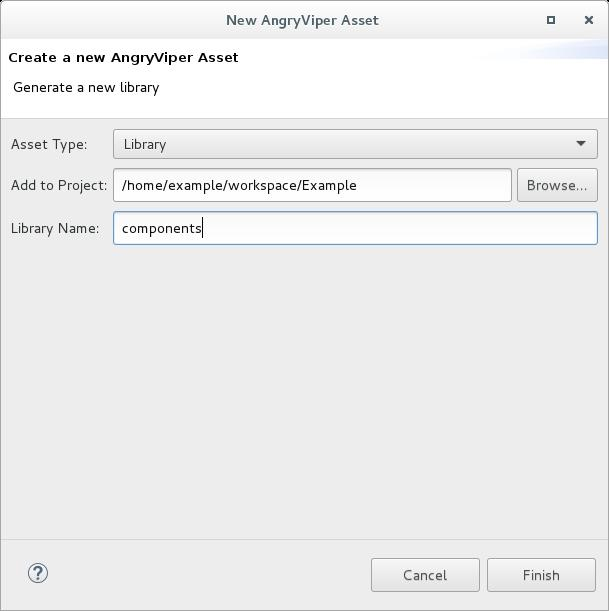
\includegraphics[scale=0.5]{figures/createlibrary.jpg}
  \caption{New OpenCPI Library Creation}
  \label{fig:figure4}
\end{figure}

\begin{figure}[h!]
  \centering
  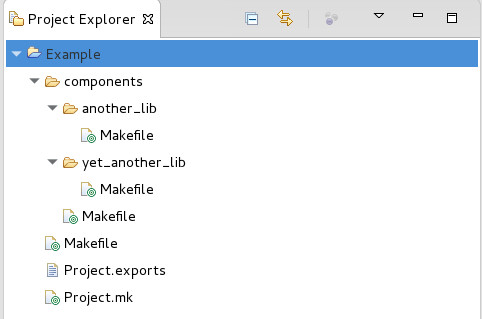
\includegraphics[scale=0.5]{figures/libraryresult.jpg}
  \caption{Library Creation Result}
  \label{fig:figure5}
\end{figure}

\end{flushleft}

\newpage

\subsection{Create New Component Spec}
\label{sec:create_spec}
\begin{flushleft}

To create a component spec within a desired project select Component from the Asset Type command drop-down list. Creating a new spec requires the user to select a project to place the spec file and input a file name. From here, the user must select whether to add this spec to the top level of the project or the default option of a specific library. The Add To Library field will provide the available library options to place this spec within the desired project. This command generates a new component spec file in the library determined above of the chosen project.\newline
\begin{figure}[h!]
  \centering
  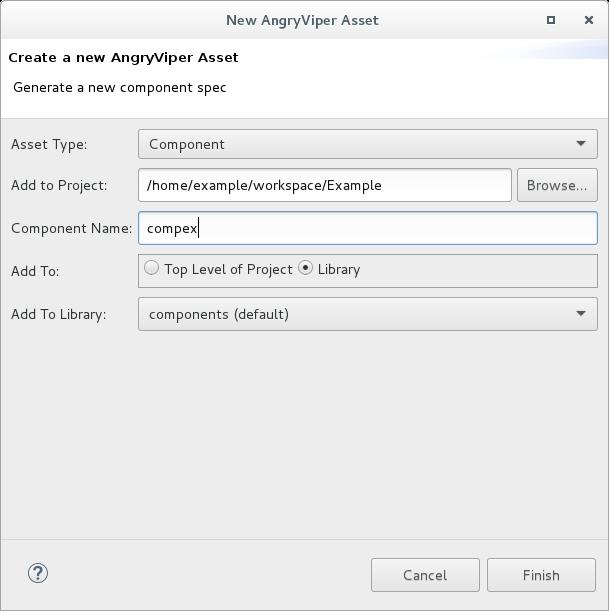
\includegraphics[scale=0.45]{figures/createspec.jpg}
  \caption{New OpenCPI Component Spec Creation}
  \label{fig:figure6}
\end{figure}

\begin{figure}[h!]
  \centering
  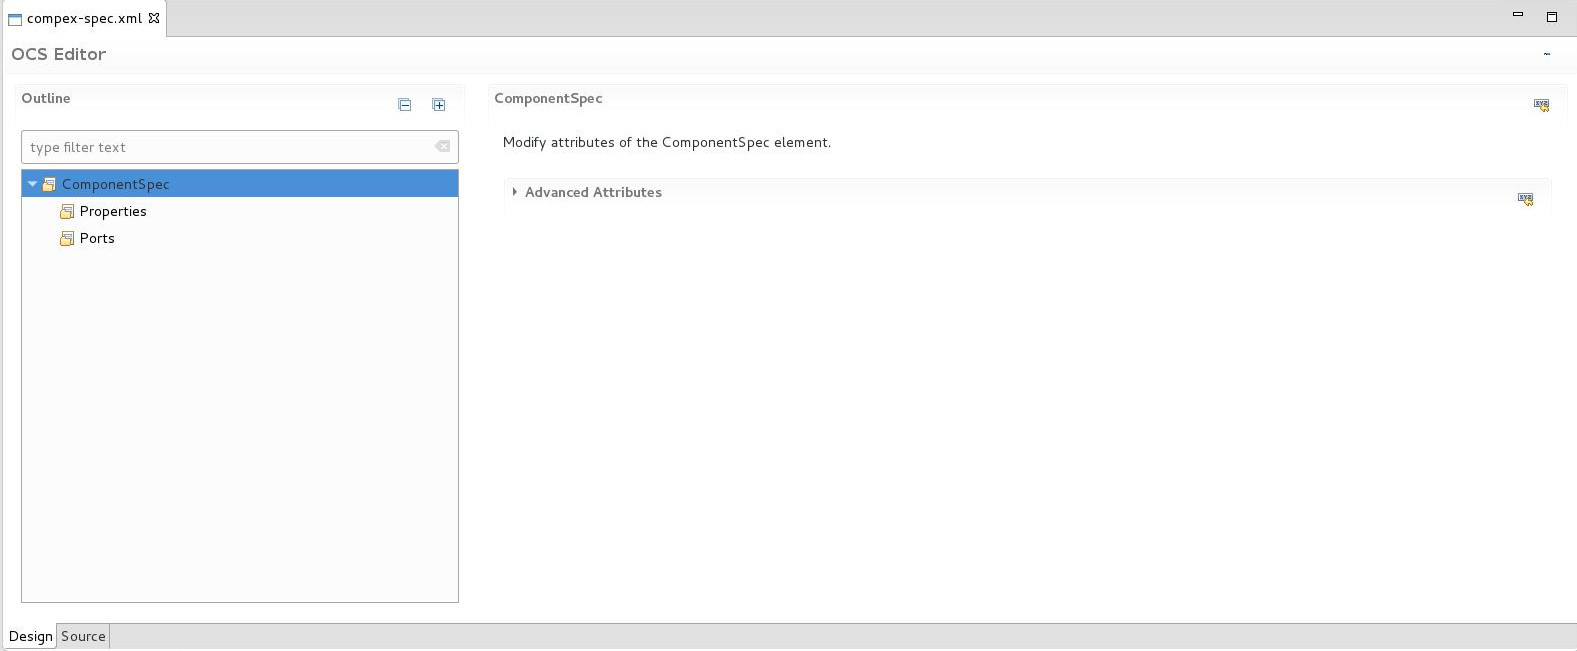
\includegraphics[scale=0.31]{figures/specresult.jpg}
  \caption{Component Spec Creation Result}
  \label{fig:figure7}
\end{figure}

\end{flushleft}

\newpage

\subsection{Create New Protocol}
\label{sec:create_protocol}
\begin{flushleft}

To create a protocol spec within a desired project select Protocol from the Asset Type command drop-down list. Creating a new protocol requires the user to select a project to place the protocol spec file and input a file name. From here, the user must select whether to add this protocol to the top level of the project or the default option of a specific library. The Add To Library field will provide the available library options to place this protocol within the desired project. This command generates a new protocol spec file in the library determined above of the chosen project.\newline
\begin{figure}[h!]
  \centering
  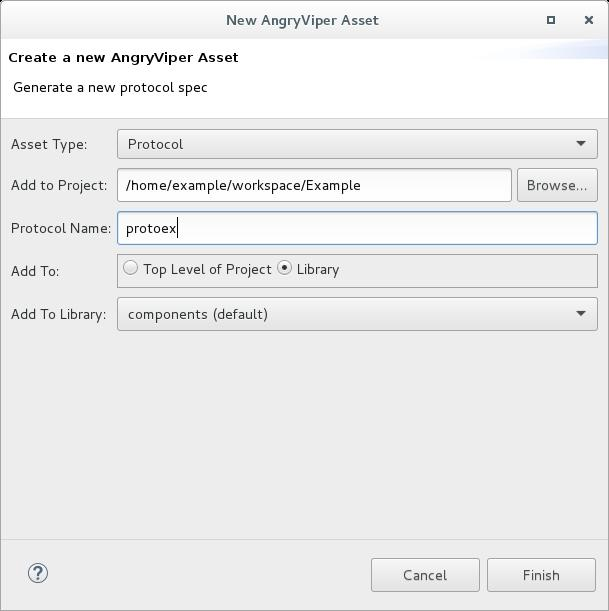
\includegraphics[scale=0.45]{figures/createprotocol.jpg}
  \caption{New OpenCPI Protocol Spec Creation}
  \label{fig:figure8}
\end{figure}

\begin{figure}[h!]
  \centering
  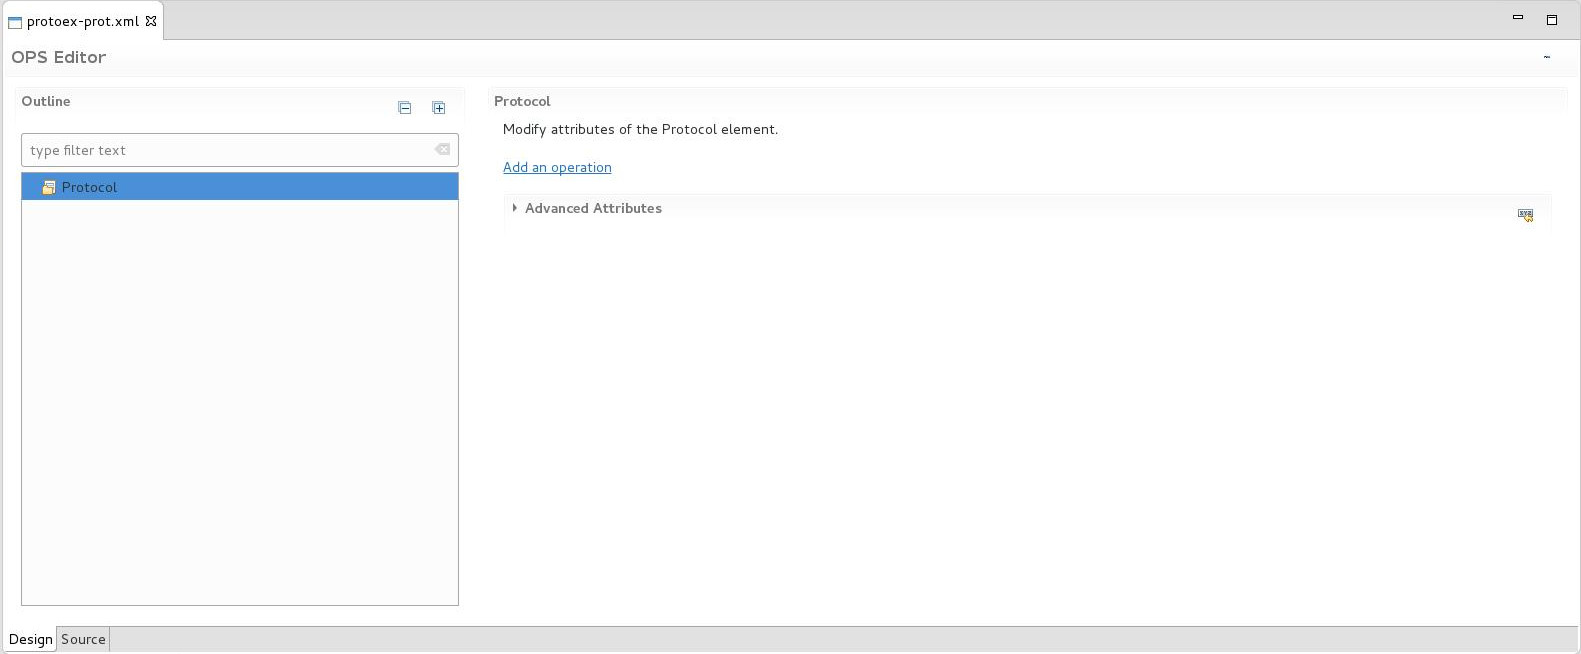
\includegraphics[scale=0.31]{figures/protocolresult.jpg}
  \caption{Protocol Spec Creation Result}
  \label{fig:figure9}
\end{figure}

\end{flushleft}

\newpage

\subsection{Create New Worker}
\label{sec:create_worker}
\begin{flushleft}

To create a worker within a desired project select Worker from the Asset Type command drop-down list. Creating a new worker requires the user to select a project to place the worker and input a worker name. This command has an Add To Library field that will provide the user with the library options for this worker in the specified project. The user must also select the spec that this worker implements as well as the authoring model and programming language. This command generates a new worker of the specified model in the library determined above of the chosen project.\newline
\begin{figure}[h!]
  \centering
  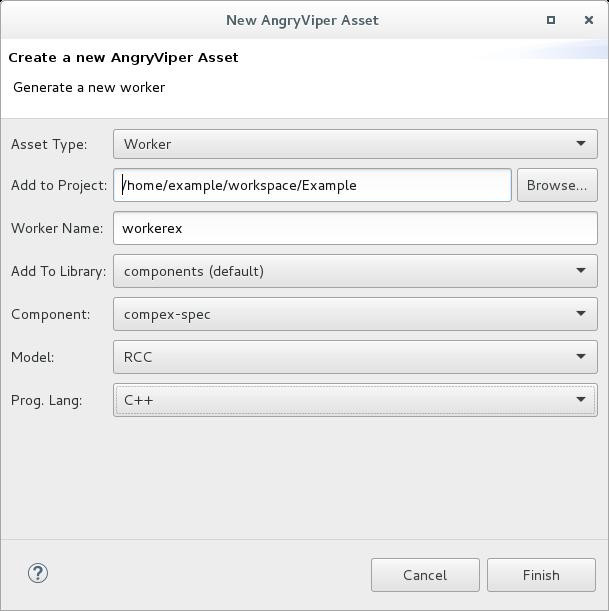
\includegraphics[scale=0.4]{figures/createworker.jpg}
  \caption{New OpenCPI Worker Creation}
  \label{fig:figure10}
\end{figure}

\begin{figure}[h!]
  \centering
  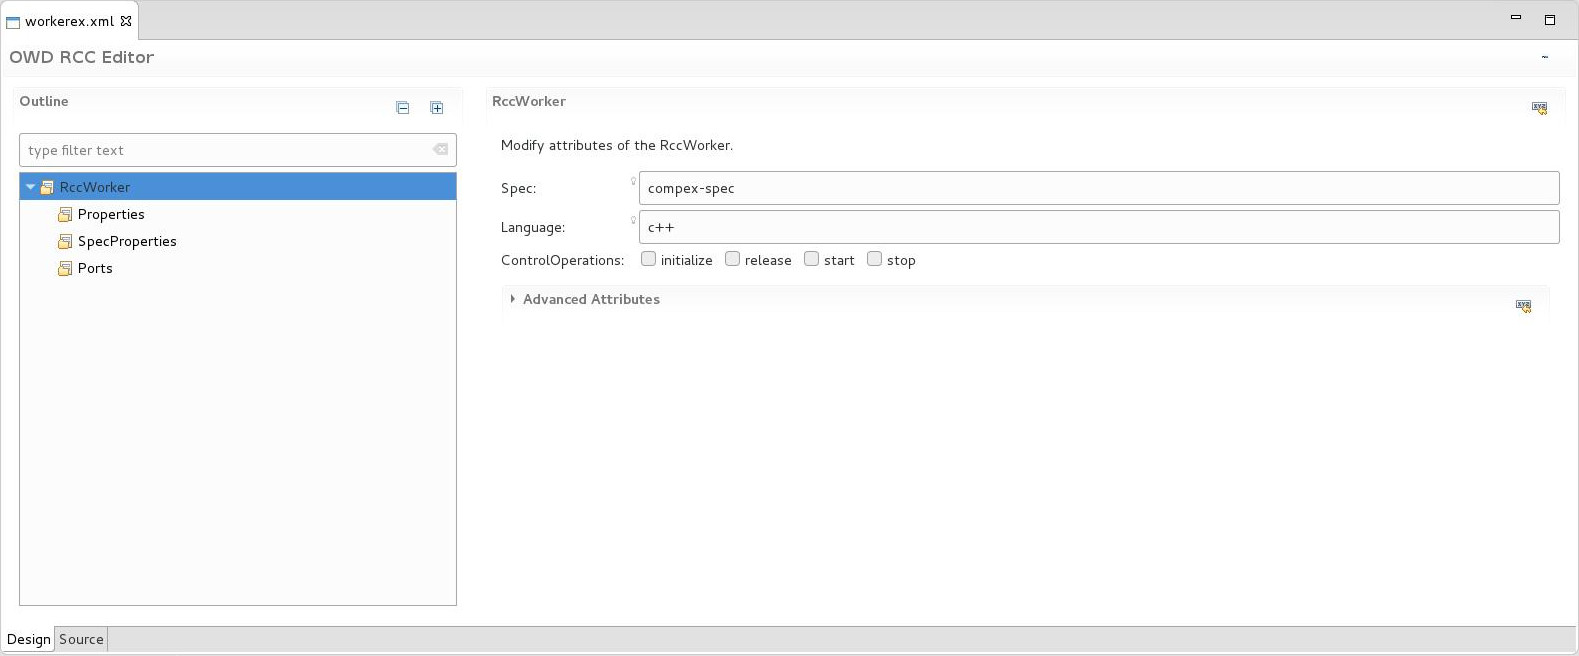
\includegraphics[scale=0.31]{figures/workerresult.jpg}
  \caption{Worker Creation Result}
  \label{fig:figure11}
\end{figure}

\end{flushleft}

\newpage

\subsection{Create New Application}
\label{sec:create_application}
\begin{flushleft}

To create an application within a desired project select Application from the Asset Type command drop-down list. Creating a new application requires the user to select a project to place the application and input an application name. There is also the optional XML Only check-box that will only create the XML file at top of the Applications folder rather than creating an application sub-folder containing the XML file \textit{and} a C++ File inside the applications folder which is the default. This command generates a new application file and/or folder inside the applications folder at the top level of the chosen project.\newline
\begin{figure}[h!]
  \centering
  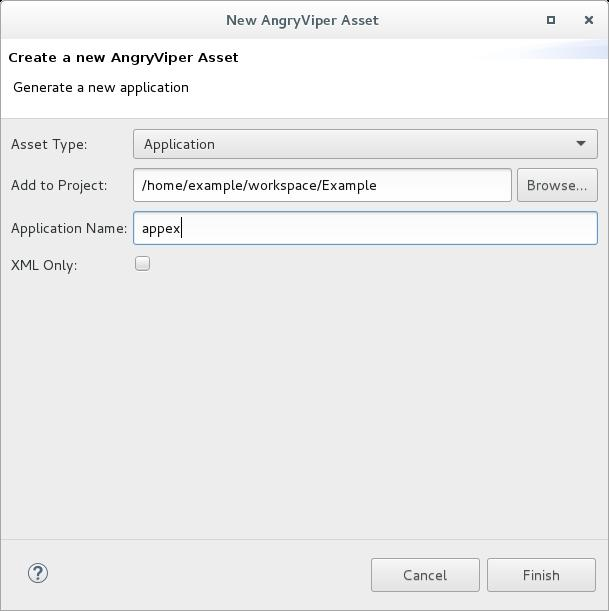
\includegraphics[scale=0.45]{figures/createapplication.jpg}
  \caption{New OpenCPI Application Creation}
  \label{fig:figure12}
\end{figure}

\begin{figure}[h!]
  \centering
  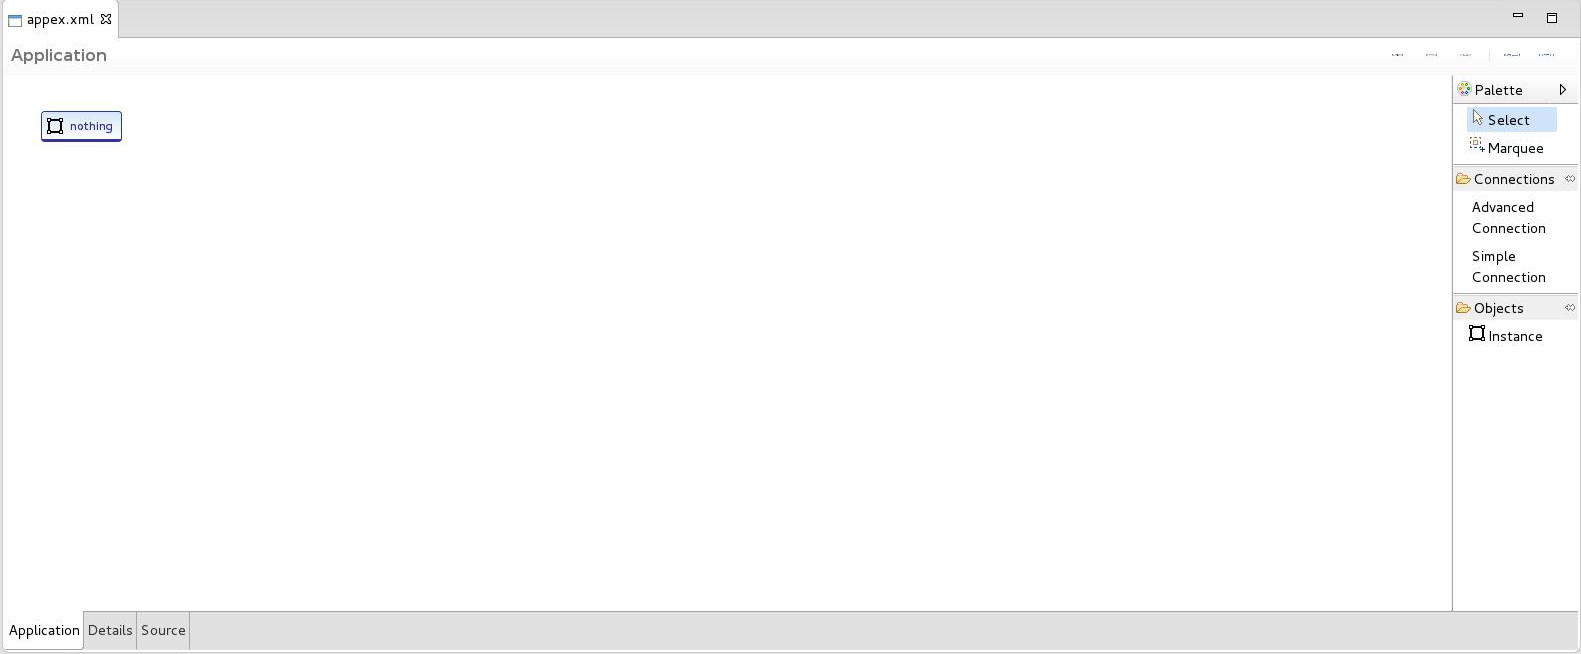
\includegraphics[scale=0.31]{figures/applicationresult.jpg}
  \caption{Application Creation Result}
  \label{fig:figure13}
\end{figure}

\end{flushleft}

\newpage

\subsection{Create New HDL Assembly}
\label{sec:create_assembly}
\begin{flushleft}

To create an assembly file within a desired project select HDL Assembly from the Asset Type command drop-down list. Creating a new assembly requires the user to select a project to place the assembly and input a file name. This command generates a new assembly folder structure inside the hdl/assemblies folder at the top level of the chosen project.\newline
\begin{figure}[h!]
  \centering
  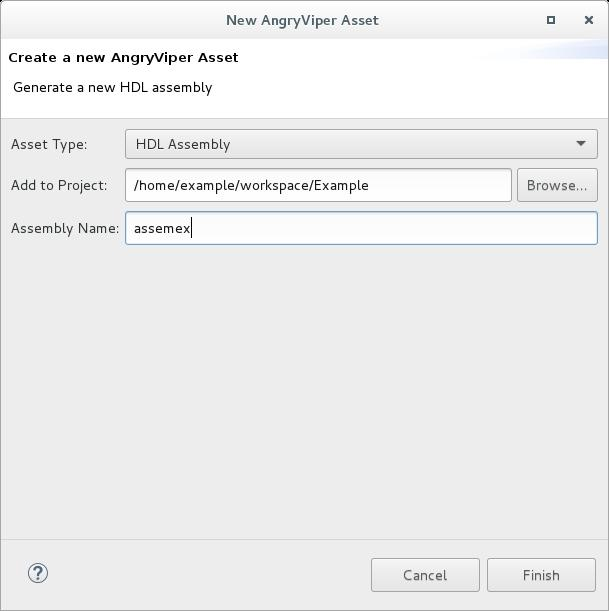
\includegraphics[scale=0.45]{figures/createassembly.jpg}
  \caption{New OpenCPI HDL Assembly Creation}
  \label{fig:figure14}
\end{figure}

\begin{figure}[h!]
  \centering
  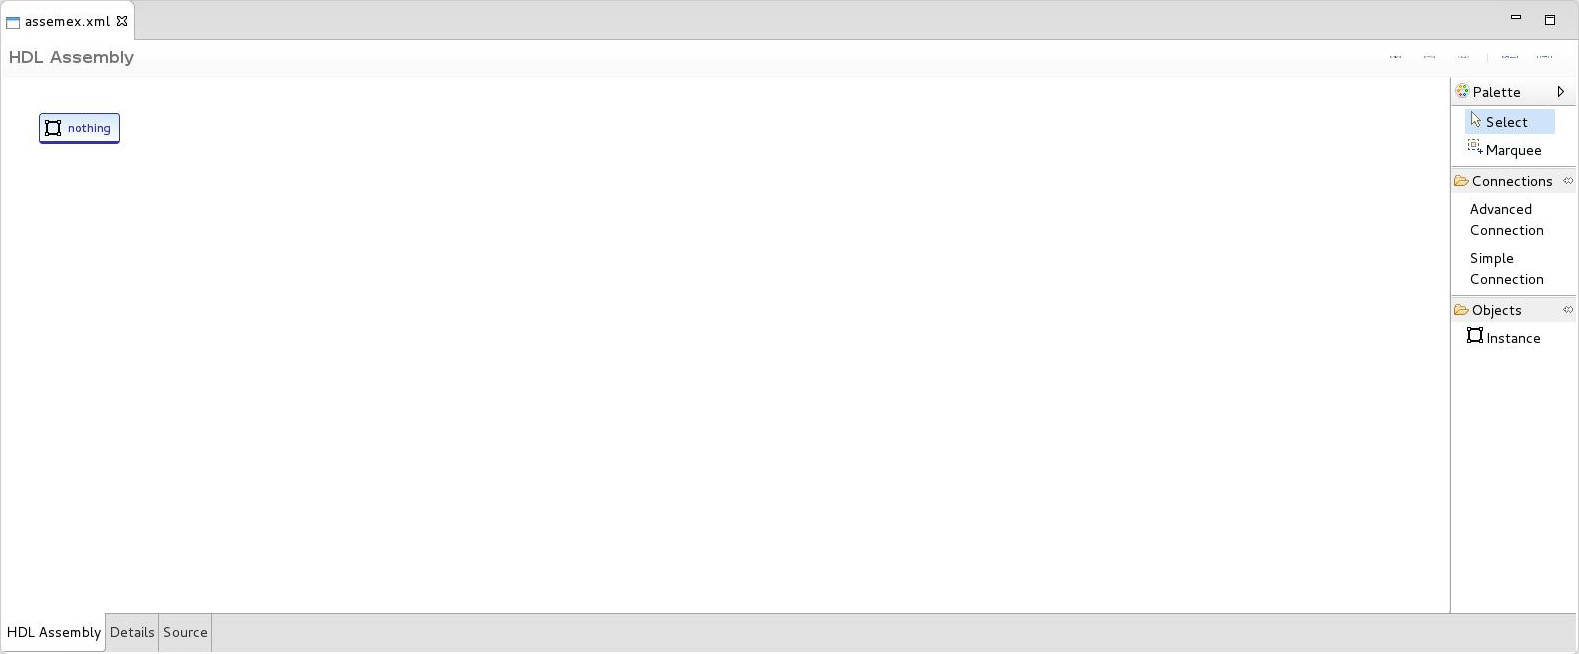
\includegraphics[scale=0.31]{figures/assemblyresult.jpg}
  \caption{HDL Assembly Creation Result}
  \label{fig:figure15}
\end{figure}

\end{flushleft}

\newpage

\section{Drag and Drop Applications and Assemblies}
\label{sec:drag_and_drop}
\begin{flushleft}

The ANGRYVIPER IDE plugin comes with a drag-and-drop feature to build and develop application and HDL assembly XML files for OpenCPI. Once an application or assembly has been created, the editors for each respective file can be used to modify them in a drag-and-drop manner. This can be seen in the images below.

\end{flushleft}

\subsection{Add Instances to Application/HDL Assembly}
\label{sec:add_application_instances}
\begin{flushleft}

To add a new Instance to the diagram, grab Instance from the Objects palette on the right side of the editor. Click and drag the new instance onto the canvas. A drop-down menu will then appear with the available specs known to this application/assembly. To change the spec associated with this instance in the future, click the name of the instance and the drop-down will reappear.

\begin{figure}[h!]
    \centering
	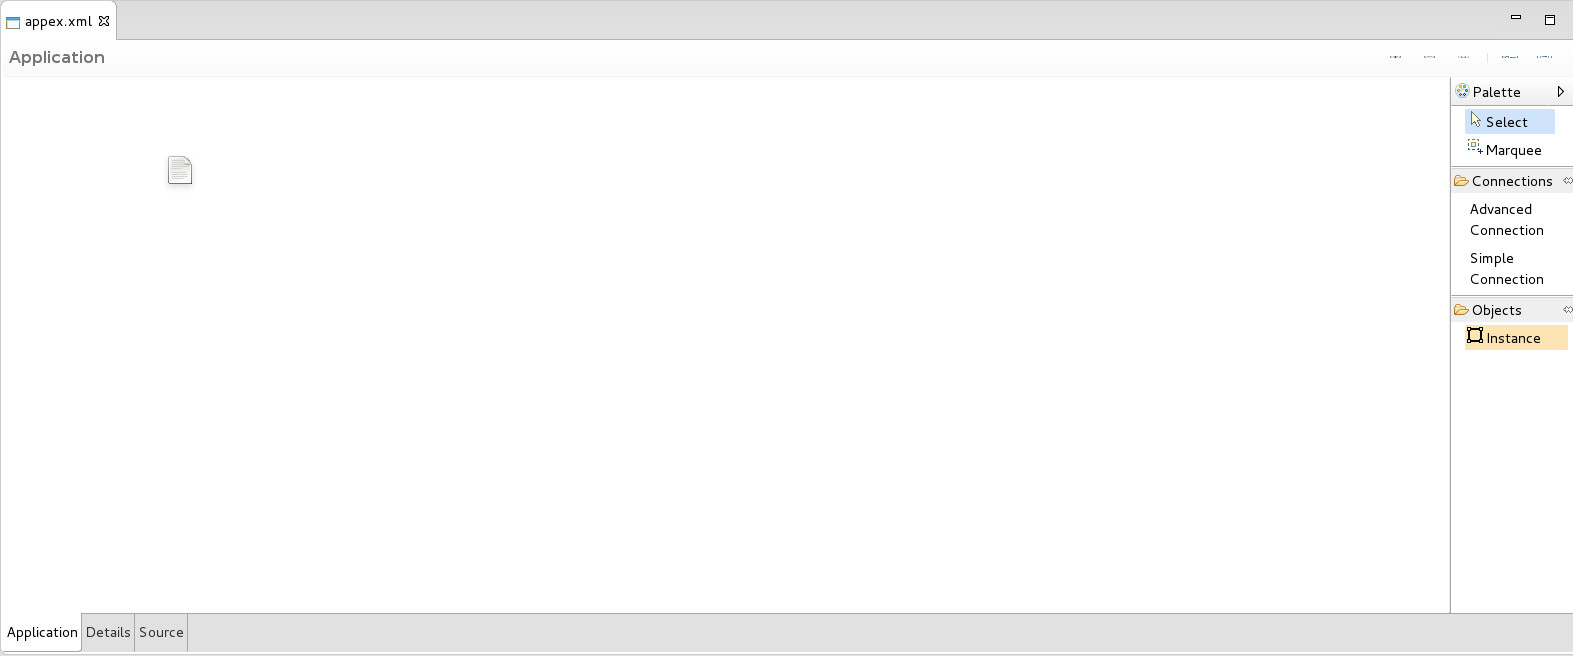
\includegraphics[scale=0.31]{figures/instance-selected.jpg}
	\caption{Select Instance from inside the Objects palette}
	\label{fig:figure16}
\end{figure}

\begin{figure}[h!]
    \centering
	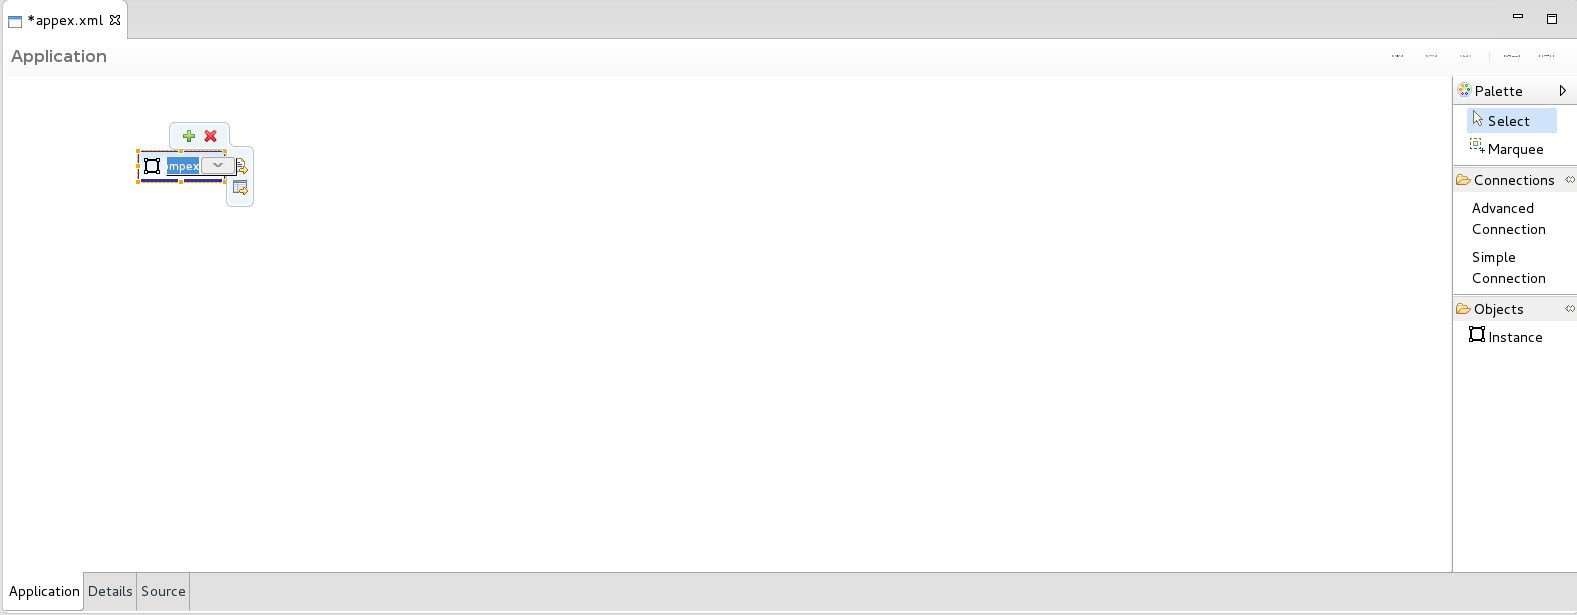
\includegraphics[scale=0.31]{figures/instance-dropped.jpg}
	\caption{Drag the Instance icon to the diagram editor and drop it at the desired location.}
	\label{fig:figure17}
\end{figure}

\begin{figure}[h!]
    \centering
	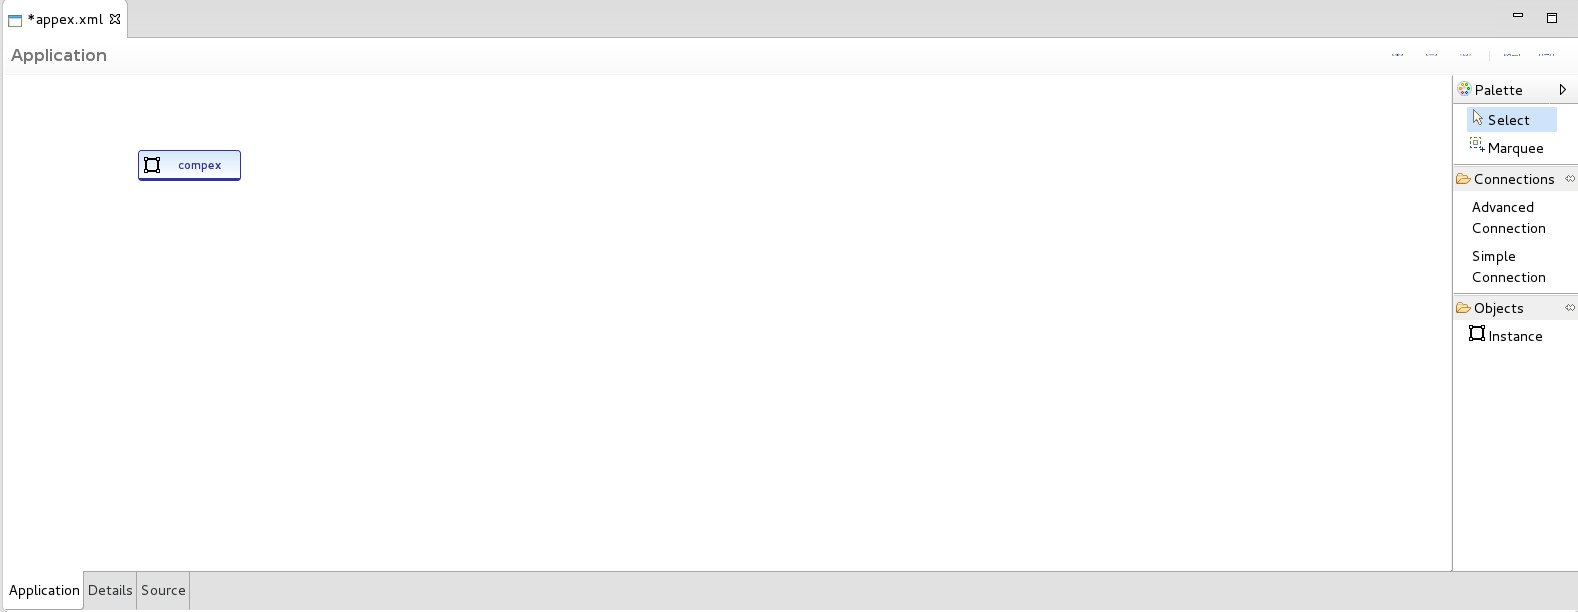
\includegraphics[scale=0.31]{figures/instance-complete.jpg}
	\caption{The new instance on the diagram}
	\label{fig:figure18}
\end{figure}
\end{flushleft}
\newpage

\subsection{Add Connections to Application/HDL Assembly}
\label{sec:add_application_connections}
\begin{flushleft}

There are two types of connections that can be made between instances. The first is a "Simple Connection" that refers to the \textit{connect} attribute of an instance. This type is used for a one-to-one connection when only one port is available for the source and target instances. The second type is an "Advanced Connection". This type is used to explicitly specify with a \textit{Connection} element which ports between the source and target instances to connect.

\subsubsection{Make a Simple Connection}
\label{sec:add_simple_connection}

\begin{figure}[h!]
    \centering
	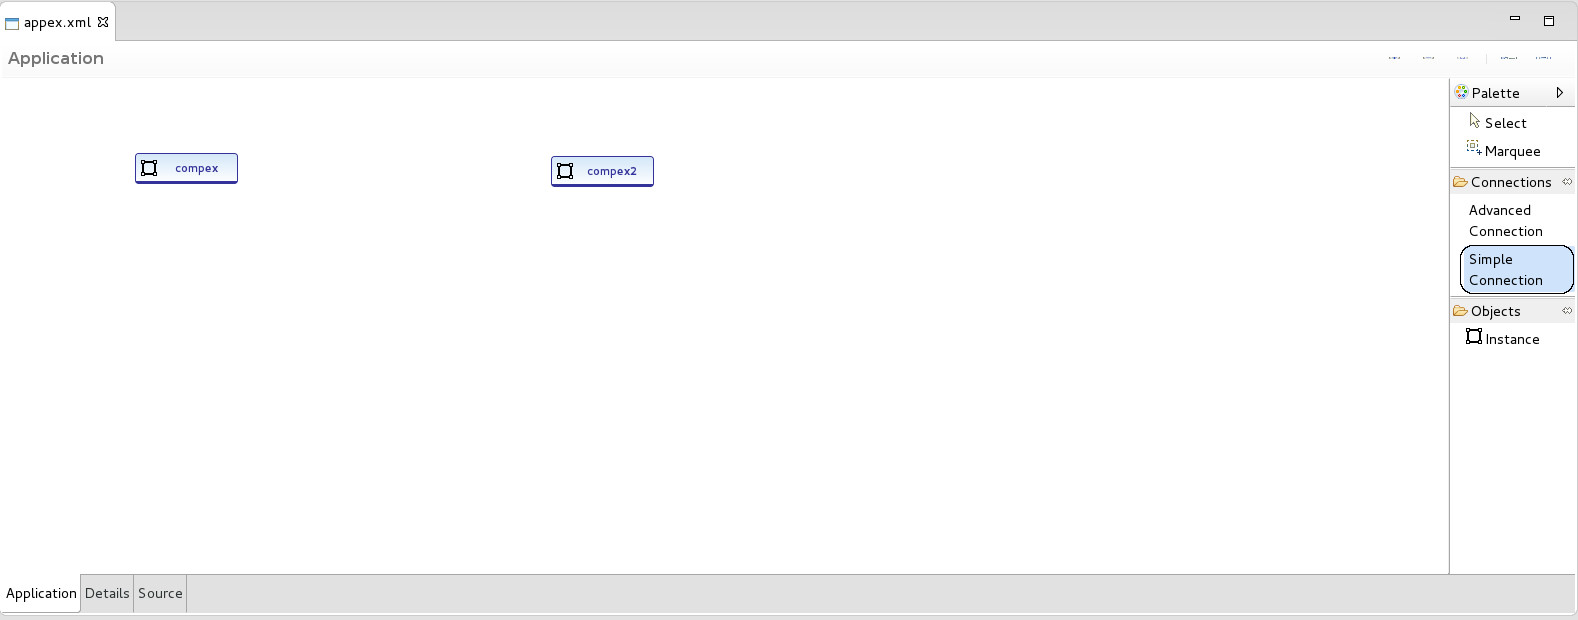
\includegraphics[scale=0.31]{figures/connect-selected.jpg}
	\caption{Select Simple Connection from the Connections palette}
	\label{fig:figure19}
\end{figure}

\begin{figure}[h!]
    \centering
	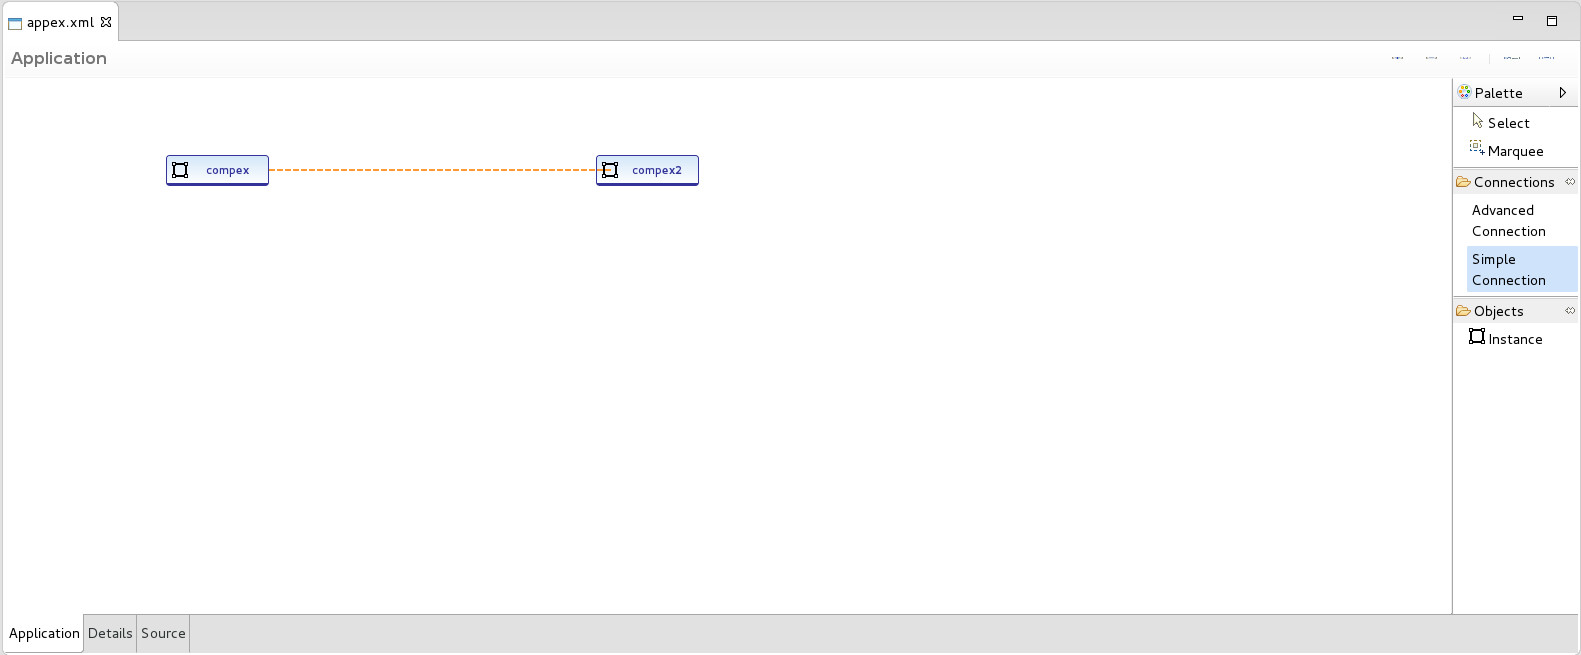
\includegraphics[scale=0.31]{figures/connect-made.jpg}
	\caption{Click the source instance followed by the target instance}
	\label{fig:figure20}
\end{figure}

\begin{figure}[h!]
    \centering
	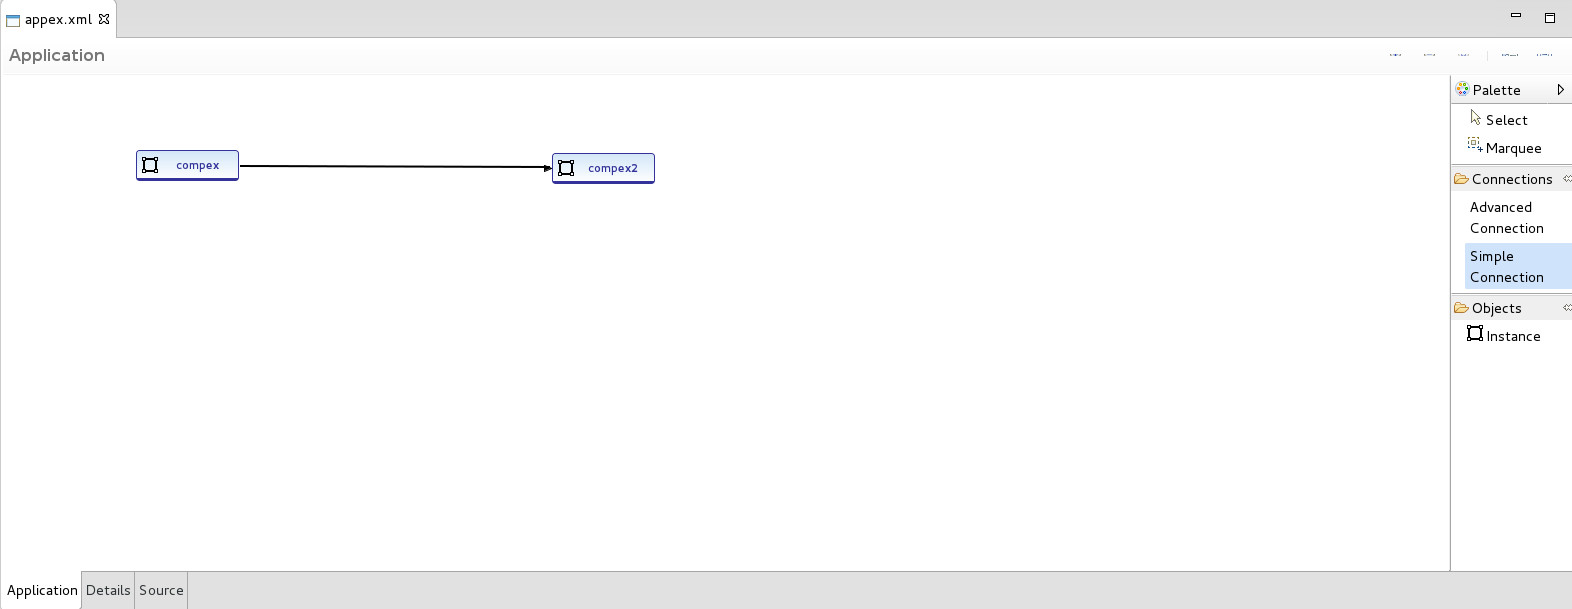
\includegraphics[scale=0.31]{figures/connect-complete.jpg}
	\caption{Simple Connection has been made between the two instances}
	\label{fig:figure21}
\end{figure}
\newpage

\subsubsection{Make an Advanced Connection}
\label{sec:add_advanced_connection}

\begin{figure}[h!]
    \centering
	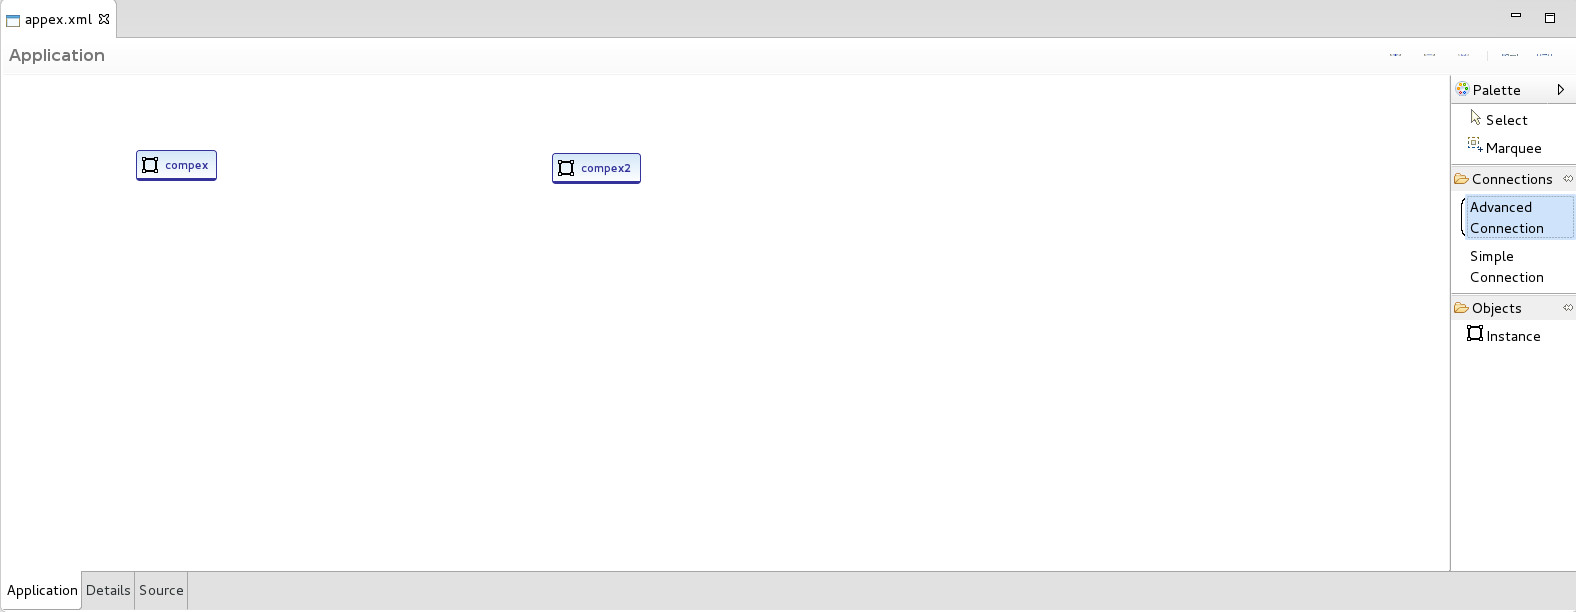
\includegraphics[scale=0.31]{figures/connection-selected.jpg}
	\caption{Select Advanced Connection from the Connections palette}
	\label{fig:figure22}
\end{figure}

\begin{figure}[h!]
    \centering
	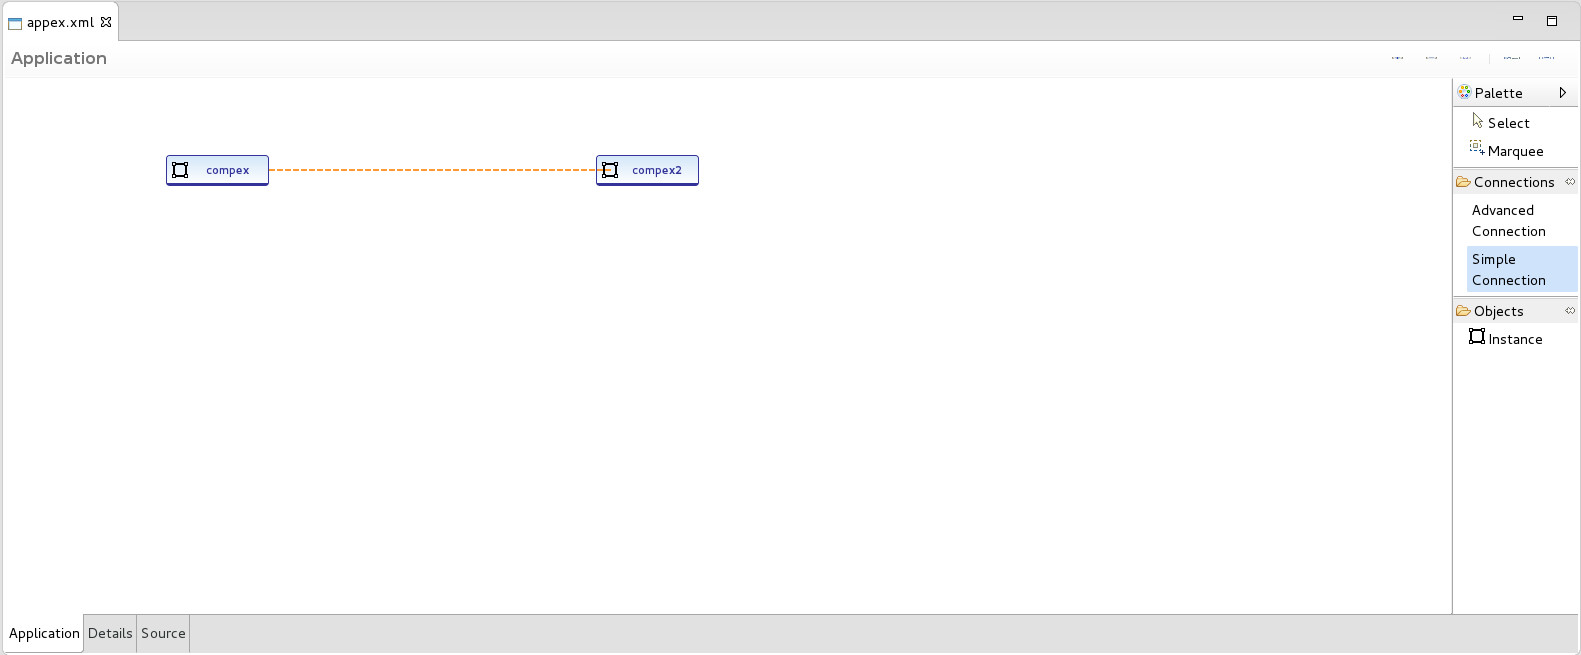
\includegraphics[scale=0.31]{figures/connect-made.jpg}
	\caption{Click the source instance followed by the target instance}
	\label{fig:figure23}
\end{figure}

\begin{figure}[h!]
    \centering
	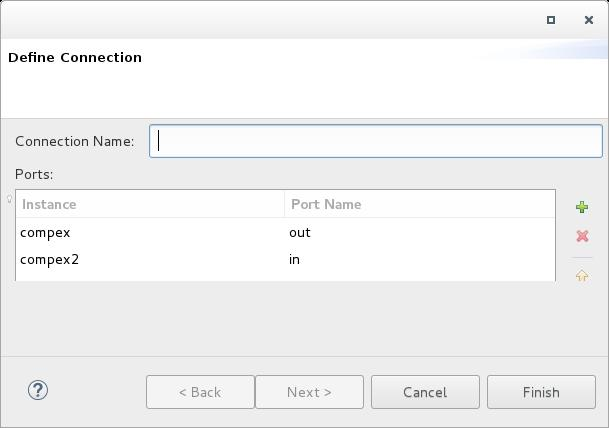
\includegraphics[scale=0.45]{figures/connection-dialog.jpg}
	\caption{Fill in appropriate information for this connection}
	\label{fig:figure24}
\end{figure}

\begin{figure}[h!]
    \centering
	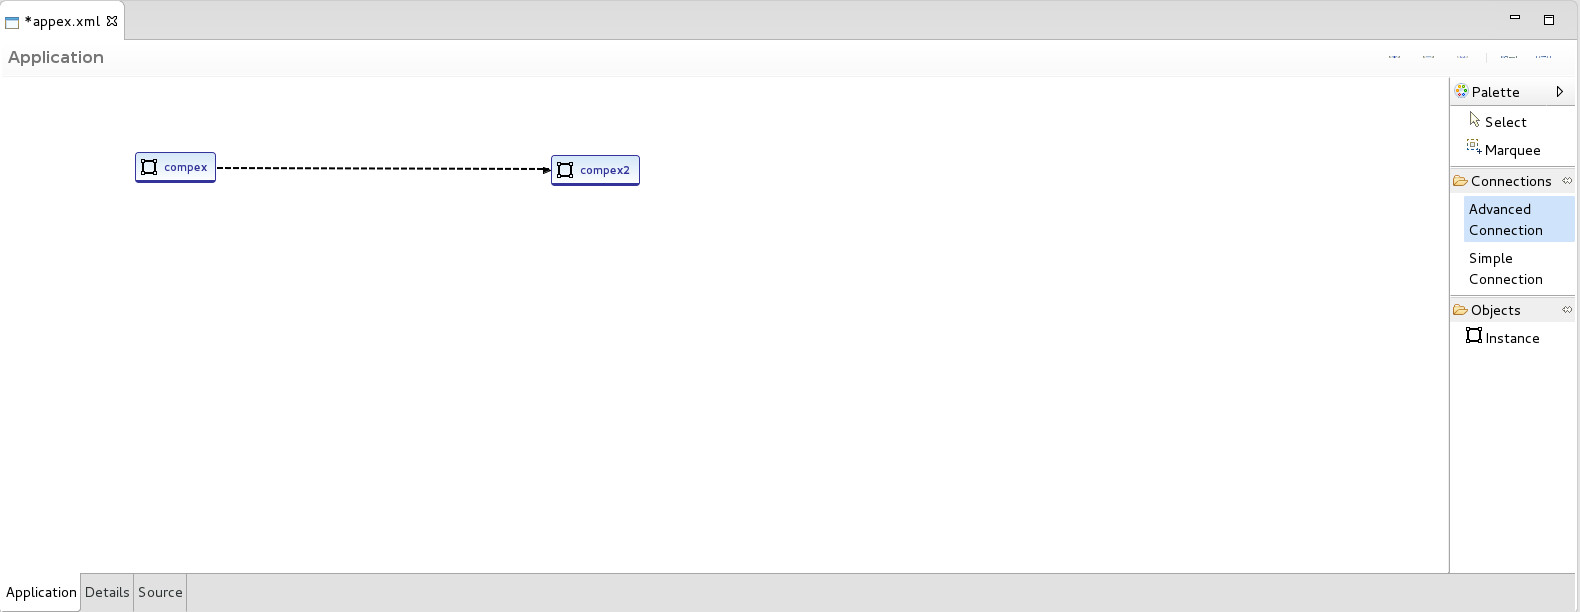
\includegraphics[scale=0.31]{figures/connection-complete.jpg}
	\caption{Advanced Connection has been made between the two instances}
	\label{fig:figure25}
\end{figure}

\end{flushleft}

\end{document}
